\documentclass{../py-lecture}

\subtitle{Introduction}

\begin{document}

\begin{frame}
  \titlepage{}
\end{frame}
\begin{frame}
  \frametitle{Outline}
  \tableofcontents{}
\end{frame}

\section{Introduction}

\begin{frame}
  \begin{block}{
      \centering\textcolor{darkgray}{What is python\ldots}}
      Python is a high-level, interpreted, interactive and object-oriented scripting language. Python is designed to be highly readable.
  \end{block}
  \vspace{.75cm}
  \hspace*{8.5cm}
\includegraphics[width=3cm]{img/python.jpg}
\end{frame}

\begin{frame}
	\frametitle{Environment}
	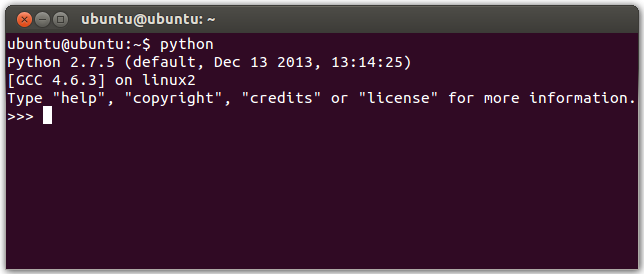
\includegraphics[width=\linewidth]{img/python-console-linux.png}
\end{frame}

\begin{frame}
	\frametitle{Variable Types}
  \begin{columns}
    \begin{column}{0.5\textwidth}
      \begin{itemize}
        \item Numbers
        \item String
        \item List
        \item Tuple
        \item Dictionary
      \end{itemize}
    \end{column}
    \begin{column}{0.5\textwidth}
	    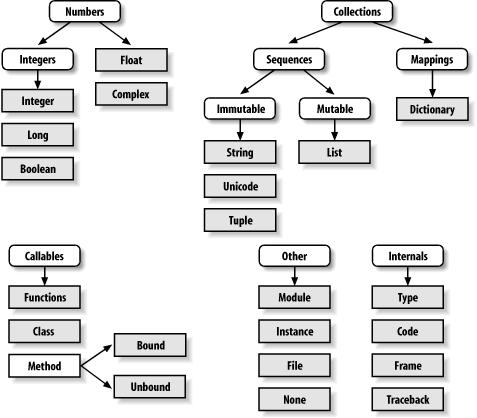
\includegraphics[width=\linewidth]{img/python-types.jpg}
    \end{column}
  \end{columns}
\end{frame}

\begin{frame}
	\frametitle{Numbers}
  \begin{itemize}
    \item Number data types store numeric values.
    \item They are immutable data types, means that changing the value of
      a number data type results in a newly allocated object.
  \end{itemize}
\end{frame}

\begin{frame}
	\frametitle{Strings}
  \begin{itemize}
    \item Strings are among the most popular types in Python.
    \item We can create them simply by enclosing characters in quotes.
    \item Python treats single quotes the same as double quotes.
  \end{itemize}
\end{frame}

\begin{frame}
	\frametitle{Lists}
  \begin{itemize}
    \item The most basic data structure in Python is the sequence.
    \item Each element of a sequence is assigned a number - its position or index.
    \item The first index is zero, the second index is one, and so forth.
  \end{itemize}
	\centering
\includegraphics[width=.4\textwidth]{img/list.jpg}	
\end{frame}

\begin{frame}
	\frametitle{Tuples}
  \begin{itemize}
    \item A tuple is a sequence of immutable Python objects.
    \item Tuples are sequences, just like lists.
    \item The differences between tuples and lists are:
    \begin{itemize}
        \item the tuples cannot be changed unlike lists
        \item tuples use parentheses, whereas lists use square brackets.
    \end{itemize}
  \end{itemize}
	\centering
\includegraphics[width=.4\textwidth]{img/tuple.jpg}
\end{frame}

\begin{frame}
	\frametitle{Dictionary}
  \begin{itemize}
    \item Each key is separated from its value by a colon (:)
    \item The items are separated by commas
    \item The whole thing is enclosed in curly braces.
  \end{itemize}
	\centering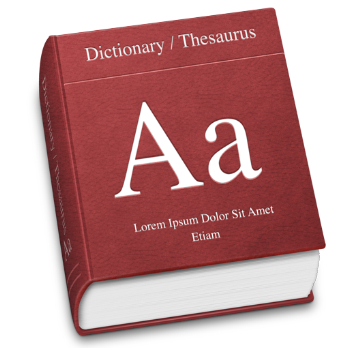
\includegraphics[width=.4\textwidth]{img/dictionary.jpg}
\end{frame}

\section{Flow Control}

\begin{frame}
	\frametitle{Flow Control}
  \begin{itemize}
    \item \mintinline{python}|if else|
    \item \mintinline{python}|for|
    \item \mintinline{python}|while|
    \item \mintinline{python}|exceptions|
  \end{itemize}
	\centering
\includegraphics[width=.4\textwidth]{img/flow-control.jpg}
\end{frame}

\section{Functions}

\begin{frame}
	\frametitle{Functions}
  \begin{itemize}
    \item Function blocks begin with the keyword \textcolor{Orange}{def},
    followed by the function name and parentheses.
    \item Any input parameters or arguments should be placed
    within these parentheses.
    \item The first statement of a function can be an optional statement -
    the documentation string of the function or docstring.
  \end{itemize}
	\centering 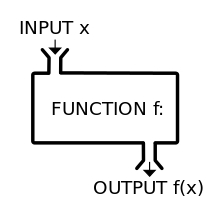
\includegraphics[width=.4\textwidth]{img/functions.jpg}
\end{frame}

\begin{frame}[fragile]
	\frametitle{Functions (Cont'd)}
  \begin{minted}[bgcolor=Black]{python}
def square(x):
    return x * x
  \end{minted}
  \begin{minted}[bgcolor=Black]{python}
def hello():
    return "Hello"
  \end{minted}
  \begin{minted}[bgcolor=Black]{python}
def printme( statement ):
    "This prints a passed string into this function"
    print statement
    return
  \end{minted}
\end{frame}

\begin{frame}[fragile]
	\frametitle{Lambda}
  \begin{itemize}
    \item Python supports simple anonymous functions through the lambda form.
    \item The executable body of the lambda must be an expression
    and can't be a statement, which is a restriction that limits its utility.
  \end{itemize}
  \begin{minted}[bgcolor=Black]{python}
foo = lambda x: x * x
  \end{minted}
	\centering 
\includegraphics[width=.3\textwidth]{img/lambda.png}
\end{frame}

\section{Classes}

\begin{frame}
	\frametitle{Classes}
  \begin{itemize}
    \item The class statement creates a new class definition.
    \item The name of the class immediately follows the keyword \textcolor{Orange}{class}
    followed by a colon as follows
  \end{itemize}
	\centering 
\includegraphics[width=.3\textwidth]{img/class.jpg}
\end{frame}

\begin{frame}[fragile]
	\frametitle{Classes (Cont'd)}
  \inputminted[bgcolor=Black,fontsize=\scriptsize,lastline=18]{python}{./src/employee.py}
\end{frame}

\begin{frame}[fragile]
	\frametitle{Classes (Cont'd)}
  \inputminted[bgcolor=Black,fontsize=\scriptsize,firstline=19]{python}{./src/employee.py}
\end{frame}

\begin{frame}
	\frametitle{Garbage Collection}
  \begin{itemize}
    \item Python deletes unneeded objects automatically to free the memory space.
  \end{itemize}
	\centering 
\includegraphics[width=.4\textwidth]{img/garbage.jpg}
\end{frame}

\begin{frame}
	\frametitle{Inheritance}
  \begin{itemize}
    \item Instead of starting from scratch, you can create a class by deriving it
    from a preexisting class by listing the parent class in parentheses
    after the new class name.
  \end{itemize}
	\centering 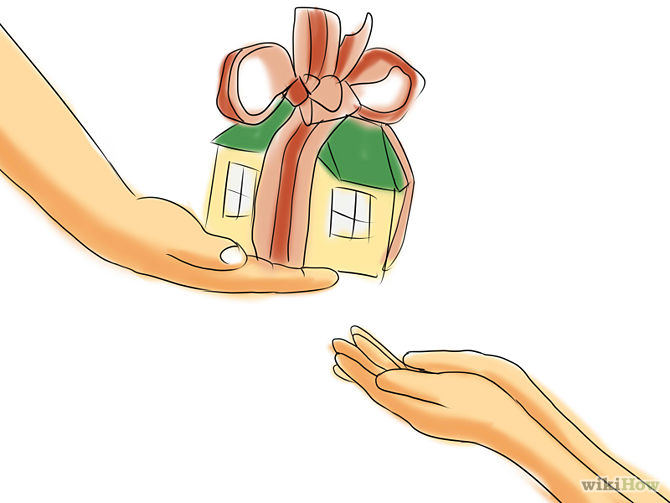
\includegraphics[width=.4\textwidth]{img/inheritance.jpg}
\end{frame}

\begin{frame}[fragile]
	\frametitle{Inheritance (Cont'd)}
  \begin{minted}[bgcolor=Black]
  {python}
class SubClassName (ParentClass1[, ParentClass2, ...]):
    """
    optional class documentation string
    """
    # class_suite
  \end{minted}
\end{frame}

\begin{frame}
	\frametitle{Special method names}
  \par
  A class can implement certain operations that are invoked by special syntax (such as arithmetic operations or subscripting and slicing) by defining methods with special names.
  \par
  This is Python’s approach to \textcolor{Orange}{operator overloading}, allowing classes to define their own behavior with respect to language operators.
\end{frame}

\begin{frame}
	\frametitle{Special method names (Cont'd)}
  \begin{itemize}
    \item \mintinline{python}|__init__( self [,args...] )| : Called after the instance has been created (by \mintinline{python}|__new__()|), but before it is returned to the caller.
    \item \mintinline{python}|__del__( self )| : Called when the instance is about to be destroyed. This is also called a finalizer or (improperly) a destructor.
    \item \mintinline{python}|__repr__( self )| : Called by the \mintinline{python}|repr()| built-in function to compute the ``official'' string representation of an object.
    \item \mintinline{python}|__str__( self )| : Called by \mintinline{python}|str(object)| and the built-in functions \mintinline{python}|format()| and \mintinline{python}|print()| to compute the ``informal'' or nicely printable string representation of an object.
    \item \mintinline{python}|__lt__( self, other )|:
    \item \mintinline{python}|__le__( self, other )|:
    \item \mintinline{python}|__eq__( self, other )|:
    \item \mintinline{python}|__ne__( self, other )|:
    \item \mintinline{python}|__gt__( self, other )|:
    \item \mintinline{python}|__ge__( self, other )|:
  \end{itemize}
\end{frame}

\begin{frame}
	\frametitle{Special method names (Cont'd)}
  \begin{itemize}
    \item \mintinline{python}|__format__(self, format_spec)|: Called by the format() built-in function, and by extension, evaluation of formatted string literals and the str.format() method, to produce a “formatted” string representation of an object.
  \end{itemize}
  \par
  The \mintinline{python}|format_spec| argument is a string that contains a description of the formatting options desired.
  The interpretation of the \mintinline{python}|format_spec| argument is up to the type implementing \mintinline{python}|__format__()|,
  however most classes will either delegate formatting to one of the built-in types, or use a similar formatting option syntax.

  \letscode{https://github.com/1995parham-learning/python101/blob/main/format/main.py}
\end{frame}

\begin{frame}
	\frametitle{Base Overloading Methods (Cont'd)}
  These methods are called to implement the binary arithmetic operations (+, -, *, @, /, //, \%, divmod(), pow(), **, <<, >>, \&, \^, |)
  \begin{columns}
    \begin{column}{.5\textwidth}
      \begin{itemize}
        \item \mintinline{python}|__add__(self, other)|
        \item \mintinline{python}|__sub__(self, other)|
        \item \mintinline{python}|__mul__(self, other)|
        \item \mintinline{python}|__matmul__(self, other)|
        \item \mintinline{python}|__truediv__(self, other)|
        \item \mintinline{python}|__floordiv__(self, other)|
        \item \mintinline{python}|__mod__(self, other)|
      \end{itemize}
    \end{column}
    \begin{column}{.5\textwidth}
      \begin{itemize}
        \item \mintinline{python}|__divmod__(self, other)|
        \item \mintinline{python}|__pow__(self, other[, modulo])|
        \item \mintinline{python}|__lshift__(self, other)|
        \item \mintinline{python}|__rshift__(self, other)|
        \item \mintinline{python}|__and__(self, other)|
        \item \mintinline{python}|__xor__ (self, other)|
        \item \mintinline{python}|__or__(self, other)|
      \end{itemize}
    \end{column}
  \end{columns}
\end{frame}

\begin{frame}
	\frametitle{Data Hiding}
			\begin{itemize}
				\item An object's attributes may or may not be visible outside \\
				the class definition.
				\item You need to name attributes with a double underscore prefix, and those \\
				attributes then are not be directly visible to outsiders.
				\item Python protects those members by internally changing the name to \\
				include the class name.
				\item You can access such attributes as \textcolor{Orange}{object.\_className\_\_attrName}
			\end{itemize}
\end{frame}

\end{document}
